\section{Planung der Datenerfassung}
Auf Grundlage des nun bekannten Systems sollen die Testfälle und Testszenarien definiert werden.

\subsection{Testszenarien}
Ein Testszenario soll das Verhalten des Netztwerks beschreiben. Ziel der in diesem Kapitel stattfindenden Untersuchung ist eine robuste Saga-Implementierung, die in allen möglichen Testszenarien ein konsistentes Verhalten des Systems gewährleistet. 

\subsection{Fehlerquellen}
Zuerst ist zu identifizieren, an welchen Stellen eine Kommunikation in einem verteilten System mittels Request-Response-Muster fehlschlagen kann. Im folgenden Beispiel wird dies anhand einer simplen Kommunikation illustriert, die aus einem Request und einer Response besteht. Es wird davon ausgegangen, dass die Verarbeitung des Requests zu einer Änderung des Systemzustands des Empfängers führt. 

\paragraph*{Szenario 1} \mbox{}\\
Im ersten Szenario entstehen keine Netzwerkfehler. Dieses Szenario ist der Ausgangspunkt. Die Korrektheit der Saga in diesem Fall ist eine Voraussetzung für die Formulierung und Analyse in folgenden Szenarien. 

\begin{figure}[H]
	\centering
	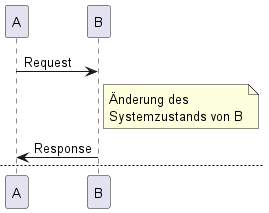
\includegraphics[width=.4\linewidth]{figures/ChapterVersuchsvorbereitung/TestSzenarien-0.png}
	\label{fig:Testszenario1}
	\caption{Sequenzdiagramm für Szenario 1}
\end{figure}
\FloatBarrier

\paragraph*{Szenario 2} \mbox{}\\
Es können Netzwerkfehler auftreten, die verhindern, dass der Request den Empfänger erreicht. Dabei findet keine Verarbeitung der Nachricht im Empfängerservice statt. Es findet weder eine Veränderung des Systemzustands des Empfängers noch eine Versendung einer Response statt.

\begin{figure}[H]
	\centering
	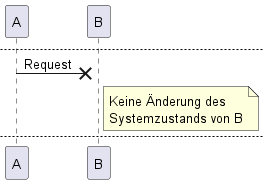
\includegraphics[width=.4\linewidth]{figures/ChapterVersuchsvorbereitung/TestSzenarien-1.png}
	\label{fig:Testszenario2}
	\caption{Sequenzdiagramm für Szenario 2}
\end{figure}
\FloatBarrier

Im Rahmen dieses Versuchs wird das Auftreten solcher Fehler in Testszenario 2 simuliert. 

\paragraph*{Szenario 3} \mbox{}\\
Findet ein Netzwerkfehler nach der Verarbeitung des Requests im Empfängerservice statt, erreicht die Response den Sender nicht. Die abgeschlossene Verarbeitung des Requests hat zu einer Veränderung des Systemzustands im Empfängerservice geführt. Dies führt dazu, dass der Sender keine Kenntnis über den Erfolg oder Misserfolg des ursprünglichen Requests hat.

\begin{figure}[H]
	\centering
	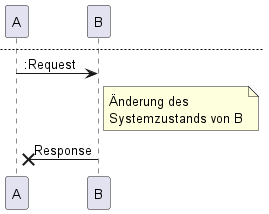
\includegraphics[width=.4\linewidth]{figures/ChapterVersuchsvorbereitung/TestSzenarien-2.png}
	\label{fig:Testszenario3}
	\caption{Sequenzdiagramm für Szenario 3}
\end{figure}
\FloatBarrier

Im Rahmen dieses Versuchs wird das Auftreten solcher Fehler in Testszenario 3 simuliert. Zusätzlich treten in Testszenario 3 die Netzwerkfehler des Testszenario 2 auf. 

Das Testszenario 3 simuliert somit ein Netzwerkverhalten, welches verschiedene Arten von Netzwerkfehlern abdeckt. Wenn eine LLT unter den im Testszenario 3 geschaffenen Bedingungen Konsistenz gewährt, kann die These angenommen werden.

% TODO

\subsection{Simulation der Testfälle} \mbox{}\\
Die zu simulierenden Testfälle werden durch einen separaten Service durchgeführt, die TestApi. Die Schnittstellen, die direkt mit der Durchführung der LLT interagieren sind:

\begin{center}
	\begin{longtable}[h]{|p{2.3cm}|p{4.9cm}|p{3.2cm}|p{3.4cm}|}
		\hline
		Service & Schnittstelle & Beschreibung & Akteur \\ \hline
		OrderService & \textit{POST /api/orders} & Platzieren einer Bestellung & Frontend (Kunde) \\ \hline
		StockService & \textit{POST /api/finish-shipment} & Lieferbestätigung & Lieferant \\ \hline
		OrderService & \textit{POST /api/cancel-order} & Stornierung & Frontend (Kunde) \\ \hline
	\end{longtable}
\end{center}
\FloatBarrier

\paragraph*{FinishOrders} \mbox{}\\
Der erste Testfall simuliert eine erfolgreiche Verarbeitung des Bestell- und Lieferprozesses. Die TestApi generiert Bestellungen und ruft den entsprechenden Endpunkt zum Platzieren im OrderService auf. Für jede der Bestellungen wird in der TestApi gewartet, bis die Lieferung ausgelöst wurde. Dann wird die Lieferbestätigung simuliert, indem der entsprechende Endpunkt im StockService aufgerufen wird. 

Der Koordinator erhält die Möglichkeit, den erfolgreichen Endzustand zu erreichen. Dies ist der erwartete Endzustand. Dieser Testfall wird als \textit{FinishOrders} bezeichnet. 

\paragraph*{CancelOrders} \mbox{}\\
Der zweite Testfall simuliert eine Stornierung der Bestellung. Die TestApi generiert Bestellungen und platziert diese. Nachdem die Lieferung ausgelöst wurde, platziert die TestApi die Stornierung. 

Der Koordinator erkennt die Stornierung und hat die Verantwortung, die Lieferung zu stoppen und im Anschluss alle lokalen Transaktionen zu kompensieren. In diesem Testfall werden alle Kompensierungen aufgerufen. Dieser Testfall wird mit \textit{CancelOrders} bezeichnet. 

Der erwartete Endzustand dieser Bestellung ist \textit{FailedWithCompensation}.
\subsection{Datengenerierung}
Um den Ablauf der Services zu simulieren, müssen Daten in jedem Teilsystem generiert werden. Dabei wird in dieser Versuchsdurchführung zwischen zwei Arten der Datengenerierung unterschieden: statische und dynamische Datengenerierung.

\paragraph*{Statisch generierte Daten} \mbox{}\\
Zu den statisch generierten Daten gehören die Daten, die manuell einmalig generiert und anschließend in die Datenbank eingefügt werden.

Im ArticleService werden die Daten der Produkttabelle generiert. Dazu gehören die verschiedenen Produktbezeichnungen und Preise.

In den zwei BankServices werden die Daten der Nutzertabellen generiert. Für jeden BankService werden 100 verschiedene Nutzer erstellt. Initial erhält jeder dieser Nutzer einen ausreichend großen Geldbetrag als Startguthaben. 

\paragraph*{Dynamisch generierte Daten} \mbox{}\\
Die in der TestApi generierten Bestellungen werden dynamisch erzeugt. Jede Bestellung wählt einen zufälligen BankService-Nutzer und eine Menge von zwischen 1 und 10 verschiedenen Artikeln mit einer zufälligen Menge zwischen 1 und 4.

Eine solche zufällig generierte Bestellung ist in \cref{lst:PlaceOrderJson} abgebildet.


\begin{lstlisting}[breaklines=true, tabsize=2, showstringspaces=false, frame=single, numbers=left, basicstyle=\small, label = {lst:PlaceOrderJson}, caption={Json für dynamisch generierte Bestellung}, captionpos=b] 
{
	"consument": {
		"userId": "Xena",
		"bankId": "Bank1"
	},
	"requestedArticles": [
	{
		"articleId": 42,
		"articlePrice": 99.0,
		"amount": 2
	},
	{
		"articleId": 16,
		"articlePrice": 49.99,
		"amount": 3
	}
}
\end{lstlisting}

\subsection{Messwerte}
Um die verschiedenen Messungen vergleichen zu können, werden die Messungen eines DEAs in jedem Testfall und in jedem Testszenario durchgeführt. Nach der Messung sollen daraus Aussagen über die Konsistenz und über die Korrektheit der modellierten LLT getroffen werden. Dazu werden folgende Messwerte erhoben:

\paragraph*{StateAnalysisResult} \mbox{}\\
Dieser Teil des Messergebnisses verwendet die im Koordinator enthaltenen Zustände. Als Scope wird ein konkreter Testfall, ein konkretes Testszenario und ein DEA festgelegt.

\begin{center}
\begin{longtable}[h]{|p{5cm}|p{12cm}|}
	\hline
	Messwert & Beschreibung \\ \hline
	totalCount & Anzahl der Sagas \\ \hline
	successfullCount & Anzahl der Sagas mit Endzustand $q_{Success}$ \\ \hline
	finishedCount & Anzahl der Sagas mit Endzustand $\not = q_{Pending}$ \\ \hline
	pendingCount & Anzahl der Sagas mit Endzustand $q_{Pending}$ \\ \hline
	failedWithCompensation\-Count & Anzahl der Sagas mit Endzustand $q_{failedWithCompensation}$ \\ \hline
	failedWithoutCompensation\-Count & Anzahl der Sagas mit Endzustand $q_{failedWithoutCompensationCount}$ \\ \hline
	hasCorrectEndstateCount & Anzahl der Sagas mit dem erwarteten Endzustand des Testfalls \\ \hline
	containsAllExpectedLogs\-Count & Anzahl der Sagas, deren Transaktionslog alle erwarteten Logs des Testfalls aufweist \\ \hline
	isSuccessfullTestInstance\-Count & Anzahl der Sagas mit dem erwarteten Endzustand und erwarteten Transaktionslogs des Testfalls \\ \hline
\end{longtable}
\end{center}
\FloatBarrier

Für jeden dieser Werte gibt wir einen normalisierter Wert berechnet, der ins Verhältnis zum Messwert \textit{totalCount} gesetzt wird. Da diese Werte ausschließlich aus der Sicht des Koordinators gemessen werden, geben diese Werte lediglich Auskunft über den erreichten Endzustand einer Saga. Eine Saga mit dem Endzustand $q_{Success}$ ist nicht gleichbedeutend mit einer konsistenten LLT. 

\paragraph*{TransactionAnalysisResult} \mbox{}\\
Um Aussagen über die Konsistenz einer LLT zu treffen, werden die durchgeführten Transaktionen, die im Transaktionslog des Koordinators festgehalten sind, mit den durchgeführten Transaktionen der Teilnehmerservices verglichen. Für jede Saga kann der Unterschied zwischen Transaktionsanzahl aus Koordinatorsicht und aus Teilnehmerservicesicht berechnet werden. Enthält eine Saga mindestens eine Transaktion, bei der dieser Unterschied auftritt, wird sie als inkonsistent bezeichnet. Die Summe der Unterschiede pro Transaktionstyp kann ebenfalls gebildet werden. Es ergibt sich folgende Tabelle:

\Needspace{5\baselineskip}
\begin{center}
	\begin{longtable}[h]{|p{5cm}|p{12cm}|}
		\hline
		Messwert & Beschreibung \\ \hline
		diffRemoveMoney\-Transaction & Summe der Unterschiede über alle Sagas für Transaktionstyp RemoveMoney \\ \hline
		diffAddMoney\-Transaction & Summe der Unterschiede über alle Sagas für Transaktionstyp AddMoney \\ \hline
		diffRemoveMoney\-CompensationTransaction &  Summe der Unterschiede über alle Sagas für Transaktionstyp RemoveMoneyCompensation \\ \hline
		diffAddMoney\-CompensationTransaction &  Summe der Unterschiede über alle Sagas für Transaktionstyp AddMoneyCompensation \\ \hline
		diffBlockArticles\-Transaction &  Summe der Unterschiede über alle Sagas für Transaktionstyp BlockArticles \\ \hline
		diffStartShipment\-Transaction &  Summe der Unterschiede über alle Sagas für Transaktionstyp StartShipment \\ \hline
		diffBlockArticles\-CompensationTransaction &  Summe der Unterschiede über alle Sagas für Transaktionstyp BlockArticlesCompensation\\ \hline
		diffStartShipment\-CompensationTransaction &  Summe der Unterschiede über alle Sagas für Transaktionstyp StartShipmentCompensation\\ \hline
		consistentSagas & Anzahl der konsistenten Sagas \\ \hline	
	\end{longtable}
\end{center}
\FloatBarrier

\paragraph*{ExecutionTimeAnalysisResult} \mbox{}\\
Schlussendlich wird ein weiteres Messergebnis definiert. Dieses Ergebnis dient dazu, die verschiedenen DEAs hinsichtlich ihrer Laufzeit zu untersuchen. Dabei wird die Differenz der ersten und letzten Transaktion im Log des Koordinators gebildet. 

\begin{center}
	\begin{longtable}[h]{|p{5cm}|p{12cm}|}
		\hline
		Messwert & Beschreibung \\ \hline
		minRuntime & minimale Laufzeit aller Sagas [s]\\ \hline
		maxRuntime & maximale Laufzeit aller Sagas [s]\\ \hline
		avgRuntime & durchschnittliche Laufzeit aller Sagas [s]\\ \hline
		medianRuntime & 50\% Quantil der Laufzeit aller Sagas [s]\\ \hline
		upperQuartileRuntime & 75\% Quantil aller Sagas [s]\\ \hline
		lowerQuartileRuntime & 25\% Quantil aller Sagas [s]\\ \hline
\end{longtable}
\end{center}
\FloatBarrier

Die Analyse der Laufzeiten trägt keine Bedeutung für Aussagen bezüglich der Konsistenz oder Korrektheit einer LLT. Ein wesentliches Werkzeug für die Definition der verschiedenen DEAs sind Retries. Die ExecutionTimeAnalysisResults geben Auskunft, inwiefern die Laufzeit einer Saga beeinflusst wird.